% Options for packages loaded elsewhere
\PassOptionsToPackage{unicode}{hyperref}
\PassOptionsToPackage{hyphens}{url}
%
\documentclass[
]{book}
\usepackage{amsmath,amssymb}
\usepackage{lmodern}
\usepackage{ifxetex,ifluatex}
\ifnum 0\ifxetex 1\fi\ifluatex 1\fi=0 % if pdftex
  \usepackage[T1]{fontenc}
  \usepackage[utf8]{inputenc}
  \usepackage{textcomp} % provide euro and other symbols
\else % if luatex or xetex
  \usepackage{unicode-math}
  \defaultfontfeatures{Scale=MatchLowercase}
  \defaultfontfeatures[\rmfamily]{Ligatures=TeX,Scale=1}
\fi
% Use upquote if available, for straight quotes in verbatim environments
\IfFileExists{upquote.sty}{\usepackage{upquote}}{}
\IfFileExists{microtype.sty}{% use microtype if available
  \usepackage[]{microtype}
  \UseMicrotypeSet[protrusion]{basicmath} % disable protrusion for tt fonts
}{}
\makeatletter
\@ifundefined{KOMAClassName}{% if non-KOMA class
  \IfFileExists{parskip.sty}{%
    \usepackage{parskip}
  }{% else
    \setlength{\parindent}{0pt}
    \setlength{\parskip}{6pt plus 2pt minus 1pt}}
}{% if KOMA class
  \KOMAoptions{parskip=half}}
\makeatother
\usepackage{xcolor}
\IfFileExists{xurl.sty}{\usepackage{xurl}}{} % add URL line breaks if available
\IfFileExists{bookmark.sty}{\usepackage{bookmark}}{\usepackage{hyperref}}
\hypersetup{
  pdftitle={Advanced decision modelling in the context of Health Technology Assessment},
  pdfauthor={Juan Pablo Diaz Martinez},
  hidelinks,
  pdfcreator={LaTeX via pandoc}}
\urlstyle{same} % disable monospaced font for URLs
\usepackage{longtable,booktabs,array}
\usepackage{calc} % for calculating minipage widths
% Correct order of tables after \paragraph or \subparagraph
\usepackage{etoolbox}
\makeatletter
\patchcmd\longtable{\par}{\if@noskipsec\mbox{}\fi\par}{}{}
\makeatother
% Allow footnotes in longtable head/foot
\IfFileExists{footnotehyper.sty}{\usepackage{footnotehyper}}{\usepackage{footnote}}
\makesavenoteenv{longtable}
\usepackage{graphicx}
\makeatletter
\def\maxwidth{\ifdim\Gin@nat@width>\linewidth\linewidth\else\Gin@nat@width\fi}
\def\maxheight{\ifdim\Gin@nat@height>\textheight\textheight\else\Gin@nat@height\fi}
\makeatother
% Scale images if necessary, so that they will not overflow the page
% margins by default, and it is still possible to overwrite the defaults
% using explicit options in \includegraphics[width, height, ...]{}
\setkeys{Gin}{width=\maxwidth,height=\maxheight,keepaspectratio}
% Set default figure placement to htbp
\makeatletter
\def\fps@figure{htbp}
\makeatother
\setlength{\emergencystretch}{3em} % prevent overfull lines
\providecommand{\tightlist}{%
  \setlength{\itemsep}{0pt}\setlength{\parskip}{0pt}}
\setcounter{secnumdepth}{5}
\usepackage{booktabs}
\ifluatex
  \usepackage{selnolig}  % disable illegal ligatures
\fi
\usepackage[]{natbib}
\bibliographystyle{apalike}

\title{Advanced decision modelling in the context of Health Technology Assessment}
\author{Juan Pablo Diaz Martinez}
\date{2021-11-05}

\begin{document}
\maketitle

{
\setcounter{tocdepth}{1}
\tableofcontents
}
\hypertarget{introduction}{%
\chapter*{Introduction}\label{introduction}}
\addcontentsline{toc}{chapter}{Introduction}

Bringing a new health technology to market and into the hands of a patient is a long process. Most of the times patients, who have a medical need, ask themselves why does it take so long to make the health technology available to everyone. When a health technology is in the market, it usually took between 5 to 10 years to make
it available.

Depending on the country, governments usually are involved in the reimbursement process. They usually ask the next questions when a new health technology is available:

\begin{itemize}
\tightlist
\item
  How much does it cost?
\item
  Will it save lives and/or improve quality of life?
\item
  Do we have enough budget to fund it?
\item
  If we have a pool of interventions for a specific disease, which one/ones should we reimburse?
\end{itemize}

Moreover, physicians, patients, insurance plans, and advocacy groups play an important role when new technologies are available in the market (why?). Even though a new technology see the light (i.e.~it has proved to be safe and effective), insurance providers or the government will not necessarily cover it. Usually they argue that the new technology is ``Not cost-effective'' or ``Not have good value for money''. \emph{These notes aim to provide all the necessary tools to decide if a new intervention has a good value-for-money.} It is important to stress that value-for-money decision is only one of many questions that are asked by one of the users of a \textbf{health technology assessment (HTA)}: patients, healthcare workers, government, and others.

\hypertarget{why-reimbursment-submissions-fail}{%
\section*{Why reimbursment submissions fail?}\label{why-reimbursment-submissions-fail}}
\addcontentsline{toc}{section}{Why reimbursment submissions fail?}

According to \citet{goeree2015health}, the reasons for rejection are:

\begin{enumerate}
\def\labelenumi{\arabic{enumi}.}
\tightlist
\item
  Inappropriate comparator. Lack of proper statistical analysis.
\item
  Inappropriate outcome. Use of surrogates.
\item
  Inappropriate analysis. Lack of robust evidence for costs and quality of life.
\item
  High cost to the government.
\end{enumerate}

\hypertarget{topics-of-the-course}{%
\section*{Topics of the course}\label{topics-of-the-course}}
\addcontentsline{toc}{section}{Topics of the course}

\begin{enumerate}
\def\labelenumi{\arabic{enumi}.}
\tightlist
\item
  What is HTA?
\item
  Introduction to decision-analytic models
\item
  Good practices in decision modelling
\item
  Evidence-based medicine
\item
  Decision tree-models
\item
  State-transition models with the Markov assumption
\item
  Partitioned survival models
\item
  Microsimulation
\item
  Discrete-event simulation
\item
  Uncertainty and decision-making
\item
  Presentation of results
\end{enumerate}

\hypertarget{statistical-computing}{%
\section*{Statistical computing}\label{statistical-computing}}
\addcontentsline{toc}{section}{Statistical computing}

The use of open-source programming languages, such as \texttt{R}, in health decision sciences is growing and has the potential to facilitate model transparency, reproducibility, and shareability. However, realizing this potential can be challenging. Models are complex and primarily built to answer a research question, with model sharing and transparency relegated to being secondary goals. Moreover, many decision modelers are not formally trained in computer programming and may lack good coding practices, further compounding the problem of model transparency. \textbf{Therefore, throughout this course, the programming language \texttt{R} will be used to show its potential for advanced modelling in the context of HTA.}

For this course, we will be using the book \href{https://r4ds.had.co.nz/}{``R for Data Science''}. To install \texttt{R} and \texttt{Rstudio}, instructions are provided in Chapter 1 of this book. We will also use Excel throughout this course.

\hypertarget{evaluation}{%
\section*{Evaluation}\label{evaluation}}
\addcontentsline{toc}{section}{Evaluation}

\begin{longtable}[]{@{}ccc@{}}
\toprule
Item & Percentage & Due date \\
\midrule
\endhead
Assignment 1 & 15\% & Nov 27, 2021 \\
Assignment 2 & 15\% & Dec 23, 2021 \\
Take-home exam & 30\% & Jan 7, 2022 \\
Project proposal & 5\% & Nov 22, 2021 \\
Project presentation & 5\% & Jan 14, 2022 \\
Final project & 30\% & Jan 17, 2022 \\
\bottomrule
\end{longtable}

The intent is to allow the students to demonstrate their mastery of this class through the following way. \textbf{Project proposal, presentation and final project will be done in pairs}.

\hypertarget{asssignments}{%
\subsection*{Asssignments}\label{asssignments}}
\addcontentsline{toc}{subsection}{Asssignments}

The assignments are handed out approximately two weeks prior to the due date. Late work will not be marked, with the exception of an advance permission from the instructor.

\hypertarget{project-proposal}{%
\subsection*{Project proposal}\label{project-proposal}}
\addcontentsline{toc}{subsection}{Project proposal}

(1 page)

The final deliverable for this course is a mini-HTA on a medical technology (preferably something topical), with a focus on the quantitative aspect of it. Given that the translation of a health policy question into a relevant research question is an essential first step in the conduct of HTA, students are required to formulate a research question and submit for grading purposes. This should include at leas some of the following: an overview of the technology being assessed; a clear specification of the policy problem; and the research question(s) (including PICO) with objectives.

\hypertarget{project-presentation}{%
\subsection*{Project presentation}\label{project-presentation}}
\addcontentsline{toc}{subsection}{Project presentation}

(20 minutes with extra 5 minutes for questions)

Students will be expected to present their final course paper and answer questions. Student will be graded on their presentations.

\hypertarget{final-project}{%
\subsection*{Final project}\label{final-project}}
\addcontentsline{toc}{subsection}{Final project}

(20 pages double-spaced)

The main assignment will require students to produce a scaled down HTA, with a focus on the quantitative aspect of it. The objective of the final project is for the student to show that they have obtained a clear understanding of the advanced methods in decision modelling in the context of HTA. More information will be provided throughout the course, but the paper should contain the following:

\begin{enumerate}
\def\labelenumi{\alph{enumi})}
\tightlist
\item
  Background and technology overview
\item
  Formulation of the question you are trying to answer through your mini-HTA
\item
  Review of the clinical literature
\item
  Description of the structure of the model
\item
  Description of the function of the model
\item
  Results
\item
  Conclusions
\end{enumerate}

\hypertarget{bibliography}{%
\section*{Bibliography}\label{bibliography}}
\addcontentsline{toc}{section}{Bibliography}

\emph{Briggs, A., Sculpher, M., \& Claxton, K. (2006). Decision modelling for health economic evaluation. Oxford University Press.}

\emph{Gray, A. M., Clarke, P. M., Wolstenholme, J. L., \& Wordsworth, S. (2011). Applied methods of cost-effectiveness analysis in healthcare (Vol. 3). Oxford University Press.}

\emph{Edlin, R., McCabe, C., Hulme, C., Hall, P., \& Wright, J. (2015). Cost effectiveness modelling for health technology assessment: a practical course. Springer.}

\hypertarget{HTA}{%
\chapter{What is HTA?}\label{HTA}}

\hypertarget{pre-session-readings}{%
\section{Pre-session readings}\label{pre-session-readings}}

\emph{Goodman, C. S. (2004). Introduction to health technology assessment. The Lewin Group. virginia, USA.} \href{https://www.nlm.nih.gov/nichsr/hta101/ta10101.html}{link}. Chapters 1, 2, and 5.

\emph{Briggs, A., Sculpher, M., \& Claxton, K. (2006). Decision modelling for health economic evaluation. Oxford University Press.} Chapter 1.

Chapters 1 and 2 of \emph{R for data science}.

\hypertarget{definition-and-rationale}{%
\section{Definition and rationale}\label{definition-and-rationale}}

The first thing that we need to know is the definition of a \textbf{health technology}. A health technology is any intervention that may be used to promote health, to prevent, diagnose or treat disease or for rehabilitation or long-term care.

\textbf{Questions}

\begin{enumerate}
\def\labelenumi{\arabic{enumi}.}
\tightlist
\item
  List some examples of health technologies.
\end{enumerate}

Depending on the agency, health technology assessment has a broad spectrum of definitions:

\emph{``HTA is a multidisciplinary process that uses explicit methods to determine the value of a health technology at different points in its lifecycle. The purpose is to inform decision-making in order to promote an equitable, efficient, and high-quality health system.'' \href{https://www.inahta.org/}{INAHTA}}

\emph{``Health technology assessment is a multidisciplinary process that uses explicit methods to determine the value of a health technology at different points in its lifecycle. The purpose is to inform decision-making in order to promote an equitable, efficient, and high-quality health system.'' \href{https://www.eunethta.eu/}{EUnetHTA}}

\emph{``A comprehensive, objective, evidence-based analysis of the clinical effectiveness, cost-effectiveness and broader impact of drugs, medical technologies and health systems. HTA examines technologies at all stages of their life cycle, from development through to maturity and obsolescence.'' \href{https://www.cadth.ca}{CADTH}}

The purpose of HTA is to support/help decision makers by identifying technologies that will improve health outcomes and deliver value for every dollar invested.

\begin{itemize}
\tightlist
\item
  Does a new health technology offer a clinical advantage over the alternatives/standard approaches?
\item
  Is it worth the investment?
\item
  Can I pay for it?
\item
  Who would benefit from it?
\item
  Any ethical, social or legal issues
\end{itemize}

But, what are the reasons for conducting HTAs?

\begin{itemize}
\tightlist
\item
  Increased demand for healthcare (why?)
\item
  Soaring healthcare costs
\item
  Increased rate of diffusion of new technologies and associated evidence
\end{itemize}

\begin{figure}

{\centering 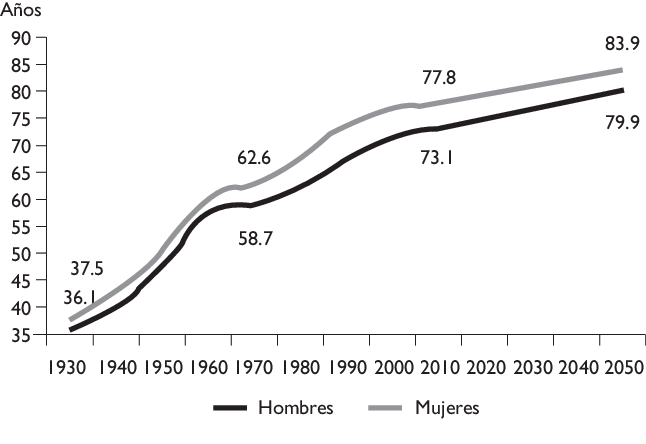
\includegraphics[width=8.97in]{images/esperanza} 

}

\caption{Life expectancy in Mexico. Source: CONAPO}\label{fig:expectancy}
\end{figure}

Once we have seen the definition and rationale for conducting HTAs, it is important to talk about the potential users.

\begin{itemize}
\tightlist
\item
  Government
\item
  Managers in hospitals
\item
  Healthcare workers
\item
  Researchers
\end{itemize}

\hypertarget{hta-process}{%
\section{HTA process}\label{hta-process}}

\begin{enumerate}
\def\labelenumi{\arabic{enumi}.}
\tightlist
\item
  Identification and prioritization of technologies
\item
  Clear specification of the problem
\item
  Technology assessment and review

  \begin{itemize}
  \tightlist
  \item
    Evidence and systematic literature review
  \item
    Aggregation and appraisal of evidence
  \item
    Synthesize and consolidate
  \item
    Collect primary data (if necessary)
  \item
    Economic evaluation, budget and health system impact
  \item
    Assessment of social, legal, and ethical consideration
  \item
    Formulation of finding
  \end{itemize}
\item
  Dissemination and implementation of recommendations
\item
  Monitor the impact of assessment reports
\end{enumerate}

\hypertarget{identification-and-prioritization-of-technologies}{%
\subsection{Identification and prioritization of technologies}\label{identification-and-prioritization-of-technologies}}

\begin{itemize}
\tightlist
\item
  Drugs seeking public or private reimbursement
\item
  Variable for non-drug technologies. However candidates:

  \begin{itemize}
  \tightlist
  \item
    High potential to improve health outcomes, reduce harm or decrease costs with similar efficacy
  \item
    Large numbers of individuals affected
  \item
    Political pressure
  \item
    Unmet needs---no current treatment
  \end{itemize}
\end{itemize}

\hypertarget{clear-specification-of-the-problem}{%
\subsection{Clear specification of the problem}\label{clear-specification-of-the-problem}}

\begin{itemize}
\tightlist
\item
  Problem statements need to consider:

  \begin{itemize}
  \tightlist
  \item
    Patient population affected (indication; epidemiology)
  \item
    Intervention being considered (drug, device, new/old)
  \item
    Comparators
  \item
    Outcome(s) or interest
  \item
    Setting (e.g.~hospital, community)
  \end{itemize}
\item
  Well formulated question
\end{itemize}

\hypertarget{technology-assessment-and-review}{%
\subsection{Technology assessment and review}\label{technology-assessment-and-review}}

\hypertarget{evidence-and-systematic-literature-review}{%
\subsubsection{Evidence and systematic literature review}\label{evidence-and-systematic-literature-review}}

\begin{itemize}
\tightlist
\item
  A comprehensive search of the literature based on systematic methods is essential
\item
  2 main types of resources relevant to HTA:

  \begin{itemize}
  \tightlist
  \item
    Published literature
  \item
    Grey literature
  \end{itemize}
\end{itemize}

\hypertarget{identification-aggregation-appraisal-of-evidence}{%
\subsubsection{Identification, aggregation \& appraisal of evidence}\label{identification-aggregation-appraisal-of-evidence}}

\begin{itemize}
\tightlist
\item
  Objective, systematic process for screening and determine studies to be included in the synthesis
\item
  Classify the studies

  \begin{itemize}
  \tightlist
  \item
    Randomised, non-randomised and economic
  \end{itemize}
\item
  Critical appraisal of the quality of the evidence
\end{itemize}

\hypertarget{synthesize-consolidate}{%
\subsubsection{Synthesize \& consolidate}\label{synthesize-consolidate}}

\begin{itemize}
\tightlist
\item
  Findings from multiple studies often combined to respond to the HTA question
\item
  Techniques commonly used to synthesize data in HTA are:

  \begin{itemize}
  \tightlist
  \item
    Meta-analysis, meta-regression
  \item
    Network meta-analysis
  \end{itemize}
\end{itemize}

\hypertarget{economic-evaluation}{%
\subsubsection{Economic evaluation}\label{economic-evaluation}}

\begin{itemize}
\tightlist
\item
  Measures the incremental costs and benefits of the technology under review compared to one or more relevant technologies
\item
  CEA, CUA and CBA
\item
  Budget impact
\end{itemize}

\hypertarget{assessment-of-social-legal-ethical-considerations}{%
\subsubsection{Assessment of social, legal \& ethical considerations}\label{assessment-of-social-legal-ethical-considerations}}

\begin{itemize}
\tightlist
\item
  Example: genetic information (why?)
\item
  Any access or equity issues following the dissemination and implementation of technologies?
\end{itemize}

\hypertarget{formulation-of-findings}{%
\subsubsection{Formulation of findings}\label{formulation-of-findings}}

\begin{itemize}
\tightlist
\item
  Explicitly link quality of the evidence to the strength of findings and recommendations as well as any limitations
\item
  Recommendations based on the findings that reflect the original question(s)
\end{itemize}

\hypertarget{dissemination-of-recommendations}{%
\subsection{Dissemination of recommendations}\label{dissemination-of-recommendations}}

\begin{itemize}
\tightlist
\item
  Findings translated into relevant and understandable information
\item
  Knowledge translation
\end{itemize}

\hypertarget{monitoring-the-impact-of-reports}{%
\subsection{Monitoring the impact of reports}\label{monitoring-the-impact-of-reports}}

\begin{itemize}
\tightlist
\item
  Some recommendations are translated into policies with clear and quantifiable impacts (e.g.~adoption of new technology, change in reimbursement)
\item
  Others go ignored and are not readily adopted into general practice
\end{itemize}

  \bibliography{book.bib,packages.bib}

\end{document}
